\documentclass[mathserif]{beamer}

\usepackage{math-19-preamble}

\usetheme{Hannover}
\usefonttheme{professionalfonts}
\usecolortheme{rose}
\usepackage{mathpazo}
\usepackage{euler}

\title{Lie groups and Lie algebras}
\subtitle{Modelling smooth symmetries}
\author{Mehek Garg, Olivia Li, Jayden Thadani, Vicente Valdes Pi\~neda}
\institute{MATH 171 --- Abstract Algebra I, Harvey Mudd College}
\date{Spring 2024}

\begin{document}
	\setbeamertemplate{sidebar left}{}

	\frame{\titlepage}

	\setbeamertemplate{sidebar left}[sidebar theme]

	\begin{frame}
		\frametitle{We will talk about}
		\tableofcontents
	\end{frame}

	\section{What Lie groups and Lie algebras are}

	\begin{frame}
		\frametitle{Manifolds}
		\only<1> {
				A smooth manifold is a generalisation of the idea of a surface. \\~
			\begin{block}{\textit{definition:} smooth manifold}
				A smooth $n$-manifold is a metric space $M$ such that every point $p \in M$ is contained in an open neighbourhood $U \subset M$ with a homeomorphism $x : U \to \mathbb{R}^{n}$. \\
			
				For overlapping $U, V \subset M$, and corresponding $x, y$, we have $x \circ y^{-1}$ smooth.
		\end{block} ~\\
	Basically every curve, surface, or region that has a well defined tangent line, plane, or space everywhere is a manifold.}
		\only<2>{	
			\begin{block}{\textit{example:} the unit circle is a $1$-manifold}
				\begin{figure}
					\centering
					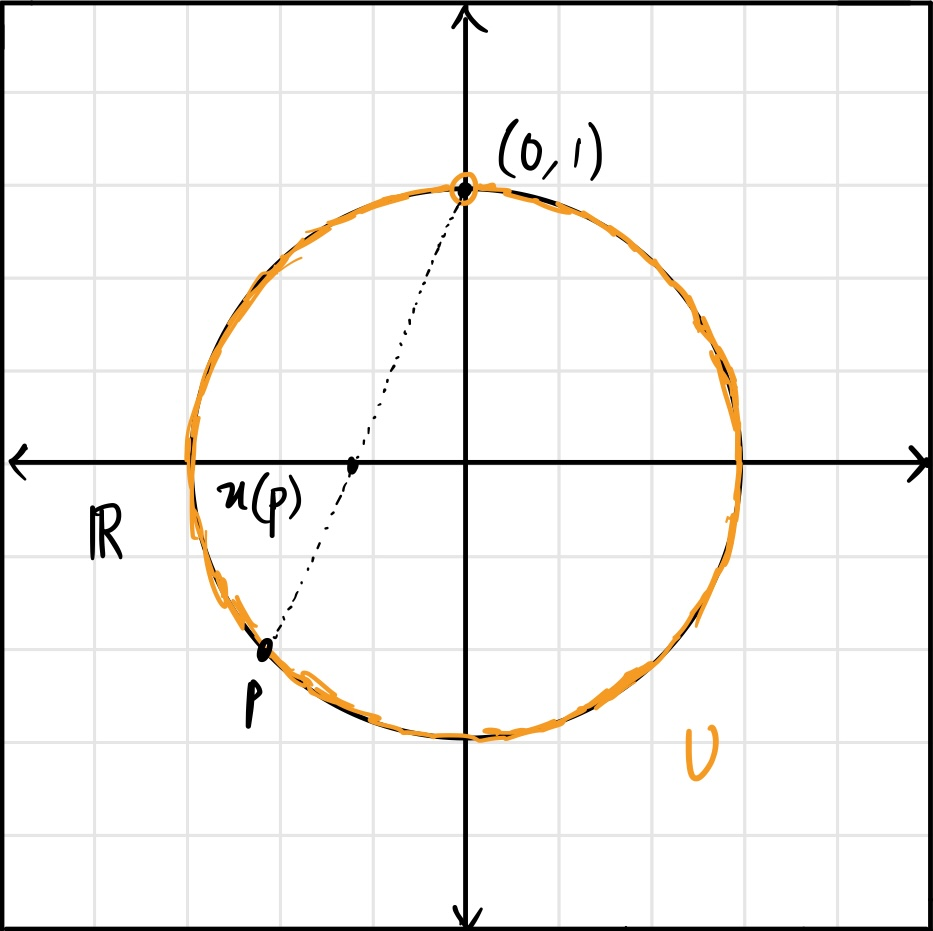
\includegraphics[width = .4\textwidth]{proj 1 unit circle} 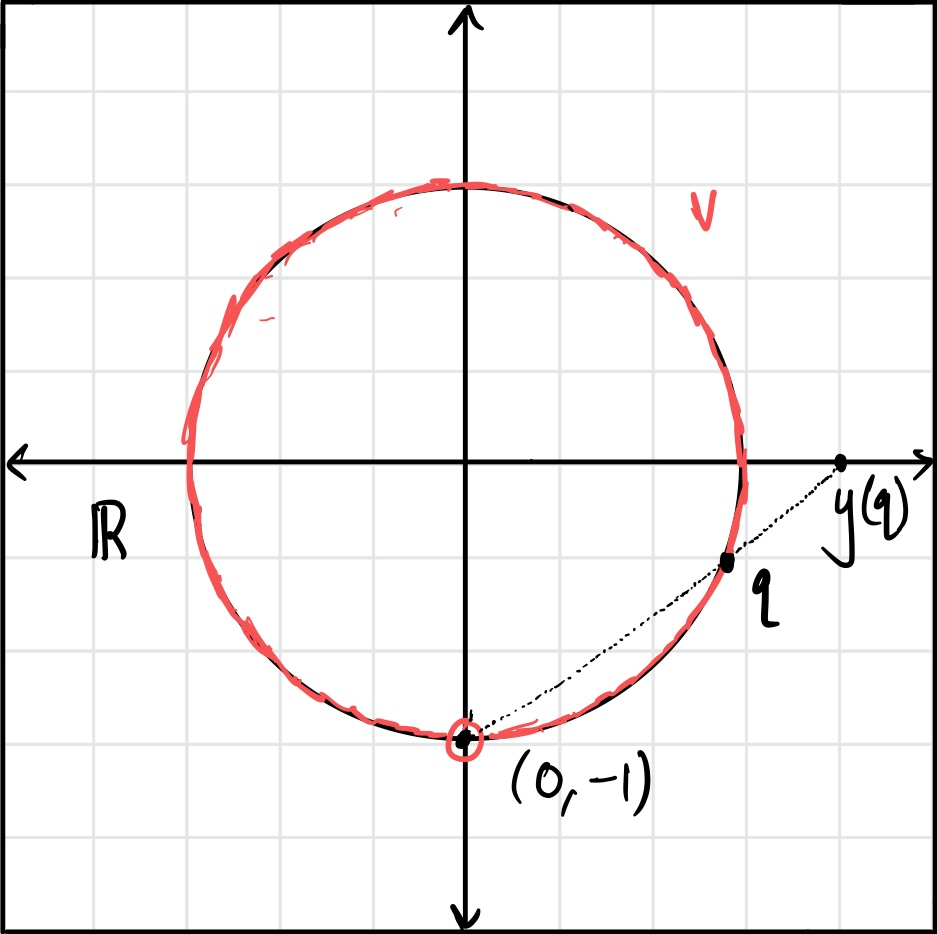
\includegraphics[width = .4 \textwidth]{proj 2 unit circle}
					\caption{$U = S^{1} \setminus \{ (0, 1) \}$ and $V = S^{1} \setminus \{ (0, -1) \}$ cover the circle and $x : U \to \mathbb{R}$ and $y : V \to \mathbb{R}$ are homeomorphisms as desired.
} 				\end{figure}
		\end{block}
		}
		\only<3>{
			But manifolds don't just have to be geometric objects. \\~
			\begin{block}{\textit{example:} the $6$-manifold of a particle}
				In physics, we often describe a particle moving in $\mathbb{R}^{3}$ by its position and momentum. This gives us a $6$-dimensional manifold that describes it completely ($3$ dimensions to describe position and $3$ to describe momentum in each direction).
			\end{block} ~\\
			The differentiable-ness of the manifold makes it particularly useful to model anything where you have variables that are constrained, but changing.
		}
	\end{frame}

	\begin{frame}{Lie groups}
		\only<1>{
			A Lie group combines the ideas of a group and a manifold. They were invented to study the smooth symmetries of differential equations. \\~
			\begin{block}{\textit{definition:} Lie group}
				A Lie group is a group $G$ that is also a smooth manifold, such that group multiplication and taking inverses are differentiable.
			\end{block} ~\\
			Basically, just like discrete groups give us \textit{moves} that retain a symmetry of an object, Lie groups give us \textit{moves} that preserve smooth symmetries. 
		}
		\only<2>{
			\begin{block}{\textit{example:} the unit circle is a Lie group}
				The unit circle $S^{1} \subset \mathbb{C}$ with the group operation given by complex multiplication is a Lie group. \\~\\
				Intuitively, this is because if we think of the derivative as the best linear approximation to the map, then multiplication by any $z \in S^{1}$ is well approximated by the linear map $w \mapsto wz$.
			\end{block}
			\begin{block}{\textit{example:} matrix Lie groups}
				If we think of $\mathrm{GL}_{n}(\mathbb{F})$ as a subset of $\mathcal{M}_{n \times n}(\mathbb{F}) \cong \mathbb{F}^{n^{2}}$, then since the zero set of the determinant is closed, $\mathrm{GL}_{n}(\mathbb{F})$ is open, and thus a submanifold. The standard operation turns out to be smooth, and thus, $\mathrm{GL}_{n}(\mathbb{F})$ is a Lie group. Similarly, other matrix groups are Lie groups too.
			\end{block}
		}
		\only<3>{
			In this presentation, we will focus on applications of examples like this one \\~\\
			\begin{block}{\textit{example:} the smooth symmetries of a differential equations}
				Consider the differential equation
				\[
					\frac{d y}{d x} = f(x)
				\]
				If $y = F(x)$ is a solution, then we call $(x, F(x))$ an integral curve. Note that $(x, F(x) + c)$ is an integral curve for any $c \in \mathbb{R}$. Thus, we have a group of symmetries isomorphic to $\mathbb{R}$, which is a Lie group.
			\end{block}
		}
	\end{frame}

	\begin{frame}
		\frametitle{Lie algebras}
		\only<1>{
			Whenever we have a complicated smooth object, it's useful to try to linearise it. Lie algebras are the linearisation of Lie groups. \\~\\
			Like any linearisation an algebra is a vector space, but it's also a ring. We can scale by elements of the base field, and multiply with $[\cdot, \cdot] : \mathfrak g \times \mathfrak g \to \mathfrak g$ as well. \\~\\
			\begin{block}{\textit{definition:} Lie algebra}
				The Lie algebra $\mathfrak{g}$ of a Lie group $G$ is the tangent space of the Lie group at the identity.
			\end{block} ~\\
			Usually, we study the simpler linear structure of the Lie algebra, and then translate back with the exponential map $\mathfrak g \to G$.
		}
		\only<2>{
			\begin{block}{\textit{example:} the Lie algebra of $S^{1}$}
				$S^{1}$ has the Lie algebra $\mathfrak{s}^{1} = (\mathbb{R}, +)$ (the real numbers with the trivial multiplication), and the exponential map by $\theta \mapsto e^{i \theta}$. 
				\begin{figure}[H]
					\centering
					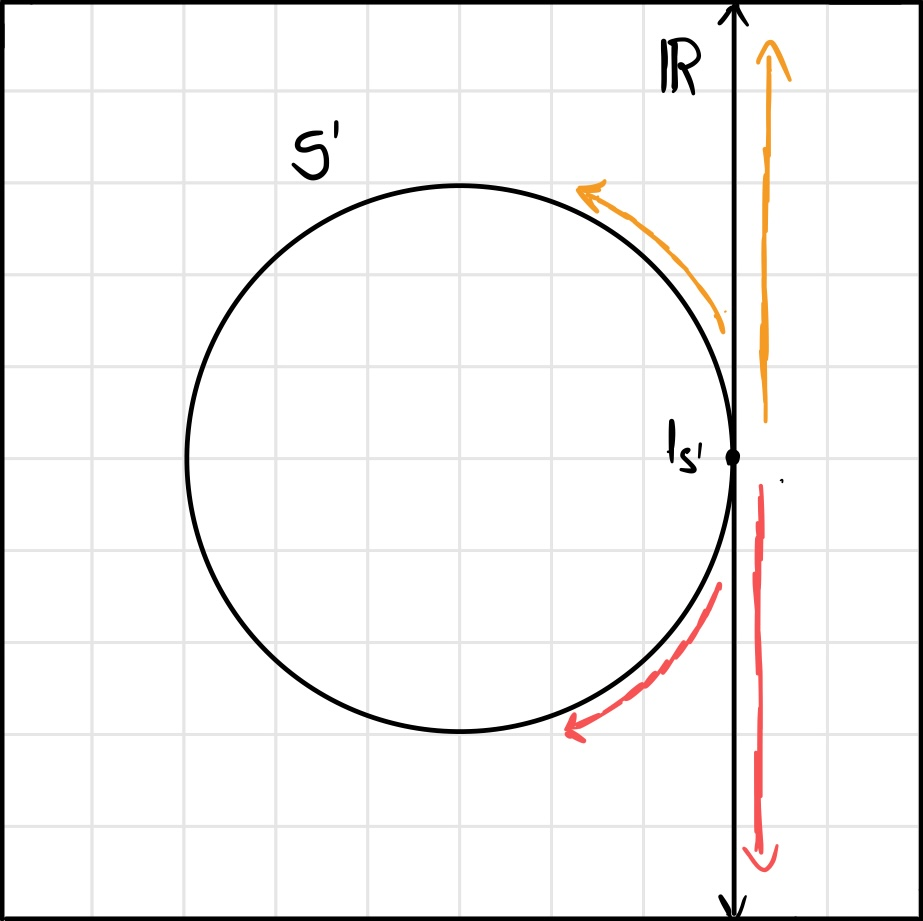
\includegraphics[width = .4 \textwidth]{lie algebra unit circle}
					\caption{$\mathfrak{s}^{1}$ represents the unit circle by adding angles!}
				\end{figure}
			\end{block}
		}
		\only<3>{
			\begin{block}{\textit{example:} the Lie algebra $\mathfrak{gl}_{n}(\mathbb{C})$ of $\mathrm{GL}_{n}(\mathbb{C})$}
				We can study $\mathrm{GL}_{n}(\mathbb{C})$ by studying all of the matrices in $\mathfrak{gl}_{n}(\mathbb{C}) = \mathcal{M}_{n \times n}(\mathbb{C})$, with the multiplication $[A, B] = AB - BA$. Since the exponential map
				\[
					\operatorname{exp} : A \mapsto I + A + \frac{A^{2}}{2!} + \dots
				\]
				always gives us a matrix $\operatorname{exp}(A)$ with nonzero determinant $e^{\operatorname{tr} A}$, we have $\operatorname{exp} : \mathfrak{gl}_{n}(\mathbb{C}) \to \mathrm{GL}_{n}(\mathbb{C})$. \\~\\
				Notice that $\operatorname{tr}(AB - BA) = 0$ and thus, $\operatorname{exp}([A, B])$ always has determinant $1$. That is, $\operatorname{exp}([A, B]) \in \mathrm{SL}_{n}(\mathbb{C})$ always. The multiplication is giving us extra information!
			\end{block}

		}
	\end{frame}

	\section{Derivative pricing}

	\section{Noether's theorem}

	\section{Particle physics}
\end{document}
